\documentclass[11pt,a4paper]{article}
\usepackage[utf8]{inputenc}
\usepackage[T1]{fontenc}
\usepackage{amsmath,amsfonts,amssymb}
\usepackage{apacite}
\usepackage{natbib}
\usepackage{graphicx}
\usepackage{booktabs}
\usepackage{threeparttable}
\usepackage{url}
\usepackage{hyperref}
\usepackage[margin=2.5cm]{geometry}
\usepackage{setspace}
\onehalfspacing

% Define \sym command for significance stars from esttab
\newcommand{\sym}[1]{{#1}}

\title{Estimating the Value of CEOs in Privately Held Businesses\thanks{Project no. 144193 has been implemented with the support provided by the Ministry of Culture and Innovation of Hungary from the National Research, Development and Innovation Fund, financed under the KKP\_22 funding scheme. This project was funded by the European Research Council (ERC Advanced Grant agreement number 101097789). The views expressed in this research are those of the authors and do not necessarily reflect the official view of the European Union or the European Research Council. \emph{Author contributions:} Conceptualization and study design: Koren, Orbán and Telegdy. Data curation, integration and quality assurance: Szilágyi and Vereckei. Statistical analysis: Koren and Telegdy. Writing the original draft: Koren. Review and editing: Koren, Orbán, Szilágyi, Telegdy and Vereckei. \emph{AI disclosure:} Claude Sonnet 4 was used to write and edit the research code and to format the manuscript (such as editing tables, figures, references, creating summaries). All code and text generated by AI tools were reviewed and edited by the authors. All authors have read and agreed to the published version of the manuscript. \emph{Data availability statement:} The data underlying this article cannot be shared publicly due to privacy and licensing restrictions. The replication package is available at \url{https://github.com/korenmiklos/ceo-value}.}}

\author{Miklós Koren\thanks{Central European University, HUN-REN Centre for Economic and Regional Studies, CEPR and CESifo. E-mail: korenm@ceu.edu} \\
        Krisztina Orbán\thanks{Monash University.} \\
        Bálint Szilágyi\thanks{HUN-REN Centre for Economic and Regional Studies.} \\
        Álmos Telegdy\thanks{Corvinus University of Budapest.} \\
        András Vereckei\thanks{HUN-REN Centre for Economic and Regional Studies, Institute of Economics.}}

\date{\today}

\begin{document}

\maketitle

\begin{abstract}
We develop a model-based approach to measure CEO value in privately held businesses, holding fixed inputs chosen by owners while substituting out variable inputs optimized by managers. Using the universe of Hungarian firms and their CEO networks over three decades (1992-2022), we estimate skill differences that translate into measurable productivity impacts. Most importantly, we develop a novel placebo-controlled event study design that reveals 73 percent of typical fixed-effect estimates reflect noise rather than true CEO effects. The naive comparison shows firms hiring better CEOs outperform those hiring worse CEOs by 25.6 percent, but placebo transitions---randomly assigned fake CEO changes excluding actual transition periods---generate an 18.8 percent spurious effect. The true causal impact is thus 6.8 percent: statistically significant and economically meaningful, but only 27 percent of the raw correlation. This methodology addresses a fundamental identification challenge in the managerial effects literature and suggests new approaches for using CEO quality measures in empirical work.
\end{abstract}

\textbf{Keywords:} CEO value, private firms, productivity

\textbf{JEL Classification:} [To be added]

\newpage

\section{Introduction}

Managers play a crucial role in determining firm performance, with effects documented across diverse institutional settings and methodological approaches. Studies using manager fixed-effects frameworks find substantial heterogeneity in managerial impact: \citet{Bertrand2003-io} show that switching from a 25th- to 75th-percentile CEO alters return on assets by about 4 percentage points in U.S. public firms, while \citet{kramarz2013thesmar} estimate CEO fixed effects in French listed companies and find that network connections significantly influence firm value. \citet{metcalfe2023managers} demonstrate that managers explain 20-30 percent of store-level sales variance in U.S. retail chains. Quasi-experimental evidence using unexpected health shocks provides causal confirmation of these large effects: \citet{bennedsen2020ceos} find that even a one-week CEO absence lowers return on assets by 7 percent in Danish private firms.

Complementary research using CEO behavioral measures and cross-country variation yields similar magnitudes. \citet{bandiera2020ceo} classify CEOs based on time-allocation patterns and show that "leader"-type managers raise firm productivity by around 8 percent across six countries, while \citet{dahlstrand2025ceo} find that "leader" CEOs boost total factor productivity by 12 percent across 42 countries, with CEO-firm mismatch costs reaching 20 percent of productivity in middle-income economies.

Despite this evidence, most existing studies face two fundamental challenges. First, they focus on publicly listed firms in developed markets, limiting applicability to the broader global economy where most businesses are privately held. Second, and more critically, standard fixed-effects approaches may substantially overstate CEO importance by failing to separate true managerial effects from spurious correlations. Recent work hints at these issues: \citet{quigley2022does} find CEO effects nearly twice as large in private versus public firms, but such estimates may conflate genuine skill differences with firm-specific trends or endogenous transition timing.

This paper makes four main contributions to address these challenges:

\textbf{First}, we develop a model-based framework to measure CEO value that explicitly separates decisions made by owners (fixed inputs like capital and organizational structure) from those made by managers (variable inputs like labor and materials). Building on \citet{Lucas1978-rp} and the decreasing returns to scale models of \citet{AtkesonKehoe2005JPE, McGrattan2012RED}, our approach identifies the marginal contribution of CEO skills to firm surplus while holding fixed the inputs chosen by owners. This theoretical clarity is essential for interpreting empirical estimates and understanding what portion of firm performance can genuinely be attributed to managerial skill.

\textbf{Second}, we implement this framework using the universe of Hungarian firms and their complete CEO network over three decades (1992-2022). This comprehensive administrative data allows us to track 960,464 firms and 665,000 unique CEOs, creating a connected network of 180,421 managers who lead multiple firms. The breadth and depth of this data---covering essentially all incorporated businesses in an entire economy over 31 years---provides unprecedented statistical power to identify manager effects and their distribution across the economy.

\textbf{Third}, we develop a novel placebo-controlled event study methodology that reveals a startling finding: approximately three-quarters of what standard fixed-effects approaches identify as CEO effects are spurious. By constructing placebo CEO transitions---randomly assigned fake transitions that exclude actual CEO change periods---we can separate true managerial impacts from noise. While the naive comparison shows firms hiring better CEOs outperform those hiring worse CEOs by 25.6 percent, placebo transitions generate an 18.8 percent effect despite no actual management change. The true causal impact is thus 6.8 percent: economically meaningful but only 27 percent of the raw correlation.

\textbf{Fourth}, we propose concrete ways researchers can address this noise problem in future work. Manager quality estimates should incorporate observable characteristics (such as foreign background or entry cohort effects) to reduce measurement error. When using CEO effects in empirical analysis, they should appear on the left-hand side of regressions where noise is less problematic, never on the right-hand side where attenuation bias dominates, and never in simple correlations where inflated variance misleads. These methodological insights have immediate practical implications for the large literature using manager fixed effects.

Our results challenge the conventional wisdom about CEO importance while providing a more rigorous foundation for understanding managerial value. The true causal effect of 6.8 percent remains substantial---replacing a 25th with a 75th percentile CEO meaningfully improves firm performance. However, recognizing that most of the apparent correlation is spurious fundamentally changes how we should measure and use CEO quality in research and practice.


\section{Modeling Framework}
Firms produce output using a Cobb-Douglas production function that incorporates both fixed and variable inputs. Owing to the presence of fixed inputs, technology exhibits decreasing returns to scale. This will pin down the scale of the firm even when markets are perfectly competitive and the firm is a price taker in both input and output markets \citep{AtkesonKehoe2005JPE,McGrattan2012RED}.\footnote{Alternatively, we could assume that firms face downward sloping residual demand curves, which would make the \emph{revenue production function} decreasing returns to scale. As long as residual demand is isoelastic, the analytical derivation of the model remains unchanged. The only difference is that the parameters have a different interpretation: the revenue elasticity of an input is the product of the input's share in revenue and $1-1/\sigma$, where $\sigma$ is the elasticity of residual demand \citep{DeLoecker2011Econometrica}.}

The production function for firm $i$ with manager $m$ at time $t$ is:
\begin{equation}
Q_{imt} = \Omega_{it}A_i Z_{m}  K_{it}^\alpha L_{imt}^{\beta} M_{imt}^{\gamma}
\end{equation}
where $\Omega_{it}$ is residual total factor productivity, $A_i$ represents time-invariant organizational capital and immaterial assets (location, brand value), $Z_m$ captures manager skill, $K_{it}$ is physical capital, $L_{imt}$ is labor input, $M_{imt}$ is intermediate input usage. The parameters $\alpha$, $\beta$ and $\gamma$ represent the elasticities with respect to physical capital, labor and material inputs, respectively. We denote $\chi := 1 - \beta - \gamma$. Conditional on productivity, organizational capital and manager skill, the production function exhibits decreasing returns to scale, $\alpha + \beta + \gamma < 1$. In a traditional production function with only capital, labor and material as inputs, $\Omega$, $A$ and $Z$ would all be lumped together as \emph{total factor productivity}.

We assume managers optimize variable inputs $L_{imt}$ and $M_{imt}$ while taking fixed inputs $A_{i}$ and $Z_m$ and physical capital $K_{it}$ as given. In private businesses, owners typically have direct control over fixed inputs, including large-scale investments in organizational and physical capital \citep{Navaretti2010EFIGE}. Managers, on the other hand, are responsible for day-to-day operations and variable input choices.

Output is sold at sector-specific price $P_{st}$, making the revenue of the firm $R_{imst} = P_{st}Q_{imt}$. The firm faces a wage rate $W_{st}$ for labor input, price $\varrho_{st}$ for intermediate inputs. After straightforward algebra solving for the optimal labor and intermediate input choices, the firm's revenue can be expressed as:
\begin{equation}\label{eq:revenue}
R_{imst} = (P_{st}\Omega_{it}A_i Z_m)^{1/\chi}
K_{it}^{\alpha/\chi}
W_{st}^{-\beta/\chi}
\varrho_{st}^{-\gamma/\chi}
(1-\chi)^{(1-\chi)/\chi}.
\end{equation}
Revenue is increasing in fixed inputs $A_i$ and $Z_m$, physical capital $K_{it}$, and decreasing in the wage rate $W_{st}$ and material input price $\varrho_{st}$. Higher prices $P_{st}$ and productivity $\Omega_{it}$ also increase revenue. Note that because $\chi<1$, the elasticity of revenue with respect to fixed inputs is greater than the elasticity in the production function, i.e. $\alpha/\chi > \alpha$. This is because the firm can leverage its fixed inputs to increase revenue more than proportionally by hiring more variable inputs.

As is usual under Cobb-Douglas production functions, the share of revenue accruing to each input is constant over time and across firms, equal to their elasticity in the production function. We define the rent accruing to fixed factors (including physical capital) 
\begin{equation}\label{eq:rent}
S_{imst} = R_{imst} - W_{st}L_{imt} - \varrho_{st}M_{imt} = \chi R_{imst}.
\end{equation}
Taking logarithms of equations \eqref{eq:revenue} and \eqref{eq:rent}, we can express the log surplus as:      
\begin{equation}\label{eq:log_surplus}
s_{imst} = C+\frac\alpha\chi k_{it} + \frac1\chi {z}_{m} + \frac1\chi p_{st} + \frac1\chi{\omega}_{it}+\frac1\chi a_i 
- \frac\beta\chi w_{st} - \frac\gamma\chi \rho_{st},
\end{equation}
where $C$ is a constant only depending on fixed parameters, $k_{it} = \ln K_{it}$, ${z}_{m} = \ln Z_m$ , $ p_{st} = \ln P_{st}$, ${\omega}_{it} = \ln\Omega_{it}$, $a_i = \ln A_i$, and $w_{st} = \ln W_{st}$, $\rho_{st} = \ln \varrho_{st}$. 

Equation \eqref{eq:log_surplus} shows how surplus depends on manager skills, holding fixed the inputs chosen by the owner and the input and output prices prevailing in the sector. Taking two managers $m$ and $m'$ with skills ${z}_m$ and ${z}_{m'}$ at the same firm, the change in surplus attributable to the new manager is:
\begin{equation}\label{eq:manager_change}
s_{im'st} - s_{imst} = \frac1\chi({z}_{m'} - {z}_{m}).
\end{equation}
The \emph{value} of the new manager to the owners of the firm is the change in surplus. This value is proportional to the difference in manager skills, scaled by the inverse of the elasticity of revenue with respect to fixed inputs $\chi$. In what follows, we aim to measure this value by estimating the change in surplus following a manager change.

\paragraph{Estimable equation.} In absence of observing organization capital and input prices, we can substitute these out with fixed effects, leading to the following estimable equation:
\begin{equation}\label{eq:estimation}
s_{imst} = \frac\alpha\chi k_{it}  + \frac1\chi\tilde{z}_m + \lambda_i + \mu_{st} + \tilde \omega_{it}
\end{equation}
where $\lambda_i = a_i/\chi$ is a firm fixed effect capturing time-invariant organizational capital, $\mu_{st} = C + p_{st}/\chi - \beta w_{st}/\chi - \gamma\rho_{st}/\chi$ is an industry-time fixed effect capturing sector-specific prices and wages, and $\tilde\omega_{it} = \omega_{it}/\chi$ is a rescaled time-varying firm productivity shock. 

Assuming that residual productivity $\tilde\omega_{it}$ is uncorrelated with manager skills and physical capital, we can estimate the model using ordinary least squares with fixed effects (OLSFE). Note that we do \emph{not} assume that manager skills are uncorrelated with physical capital, organizational capital or sectoral prices. It may well be the case that better firms with good price conditions hire better managers and invest more. 

Given our estimated parameters and fixed effects, we can recover manager skills as:
\begin{equation}\label{eq:estimated}
\hat\chi s_{imst} -  \hat\alpha k_{it}  -\hat\chi \lambda_i -\hat\chi \mu_{st} := \tilde s_{imst} = \hat z_m + \hat\omega_{it}. 
\end{equation}
We remove the contribution of physical capital, firm and industry-year fixed effects from log surplus to obtain a \emph{residualized surplus} $\tilde s_{imst}$. Because $\omega_{it}$ is assumed to be mean zero independent of $m$, we can estimate $\hat z_m$ as the average of $\tilde s_{imst}$ across all observations for manager $m$. This gives us a consistent estimate of manager skill, $\hat z_m = \frac1{N_m}\sum_{i,t} \tilde s_{imst}$, where $N_m$ is the number of observations for manager $m$.\footnote{This is equivalent to including a manager fixed effect in the regression, similar in spirit to \citet{Abowd1999Econometrica} and \citet{Card2018JoLE}. This notation emphasizes that manager effects estimated from fewer observations are noisier.}

\section{Data and Measurement}
\paragraph{Main data sources.} Our analysis uses comprehensive administrative data on Hungarian firms during 1992-2022, created by merging balance sheet and financial statement data with firm registry information. The balance sheet data come from \citet{merleg2024} and contains financial information for essentially all Hungarian firms required to file annual reports. The firm registry data come from \citet{cegjegyzek2024} and includes information on firm registration, ownership structure, and director appointments. Both datasets are distributed by HUN-REN KRTK and originally published by Opten Zrt.\footnote{The data cannot be publicly shared due to privacy and licensing restrictions. The replication package available at https://github.com/korenmiklos/ceo-value describes how to get access to the data.}

The balance sheet data include all firms required to file financial statements with Hungarian authorities, covering essentially the entire formal business sector except for the smallest corporations not engaged in double-entry bookkeeping and individual entrepreneurs. The dataset contains detailed financial information including sales revenue, export revenue, employment, tangible and intangible assets, raw material and intermediate input costs, personnel expenses, and ownership indicators for state and foreign control.

Registry information is collected by the Hungarian Corporate Court, which maintains legally mandated public records on firms \citep{cegtv}. These records include information on company representatives---individuals authorized to act on behalf of the firm in legal and business matters. Representatives may include CEOs and other executives, but also lower-level employees with signatory rights. We exclude the rare instances where the representative is a legal entity. The dataset is structured as a temporal database: each entry has an effective date interval and reflects the state of representation at a given time. Updates occur not only when positions change but also when personal identifiers (e.g., address) are modified or when reporting standards evolve. Start and end dates are often missing, and prior to 2010, the data does not contain unique numerical identifiers for individuals.

We resolve individual identities by linking records based on name, birth date, mother's name, and home address, creating a unique identifier for each person. This entity resolution step enables tracking of representatives over time and across firms. To construct an annual panel of top managers, we infer the period of service for each representative using available date bounds and sequential information. A representative is considered active in a given year if their tenure includes June 21 of each year.

Because job titles are not standardized, identifying the CEO requires heuristic rules. When an explicit title such as \emph{managing director} is available, we classify the individual accordingly. For firms lacking such labels, we assume that all representatives are CEOs if the number of representatives is three or fewer. If there are more than three and one of them was previously identified as a CEO, we assign the CEO role based on continuity. This approach allows us to systematically identify the firm's top executive across years.

\paragraph{Sample construction.} We construct our analytical sample through several filtering steps. We restrict our analysis to the period 1992 to 2022 to focus on the post-transition Hungarian economy. This removes 136,141 observations from years prior to 1992, when the economic and institutional environment was fundamentally different. Our sample contains 10,214,120 firm-year observations spanning 31 years. Table \ref{tab:sample} shows the temporal distribution of observations in our final sample. The sample exhibits steady growth from 98,780 observations in 1992 to 454,106 in 2022. This expansion reflects the growth of entrepreneurship in Hungary following the transition to a market economy.

\begin{table}[htbp]
\centering
\caption{Sample Over Time}
\label{tab:sample}
\begin{tabular}{*{6}{c}}
\toprule
Year & \shortstack{Total\\firms} & \shortstack{Sample\\firms} & CEOs & \multicolumn{2}{c}{Connected component} \\
\cmidrule(lr){5-6}
 & & & & Firms & CEOs \\
\midrule
1992 &       98,780 &       25,833 &       31,746 &        1,423 &        1,713 \\
1995 &      171,759 &       45,828 &       53,704 &        2,659 &        3,028 \\
2000 &      280,386 &       73,837 &       83,862 &        4,783 &        5,100 \\
2005 &      326,905 &       92,242 &      104,380 &        6,283 &        6,474 \\
2010 &      384,570 &      103,892 &      116,680 &        7,405 &        7,084 \\
2015 &      433,371 &      116,543 &      124,960 &        8,332 &        7,488 \\
2020 &      424,501 &      115,755 &      123,504 &        7,789 &        6,841 \\
2022 &      454,106 &      113,387 &      121,730 &        7,419 &        6,509 \\
\midrule
Total &    1,063,172 &      217,737 &      339,993 &       14,416 &       22,001 \\
\bottomrule
\end{tabular}
\begin{minipage}{12cm}
\footnotesize
\textit{Notes:} This table presents the evolution of the sample from 1992 to 2022. Column (1) shows the total number of distinct firms with balance sheet data. Column (2) shows the number of distinct firms after applying data quality filters. Column (3) shows the number of distinct CEOs. Columns (4) and (5) show the subset of distinct firms and CEOs that belong to the largest connected component of the manager network, where managers are connected if they have worked at the same firm. The table shows every fifth year plus the first year (1992), last year (2022), and totals of distinct counts. \end{minipage}
\end{table}


\textbf{CEO panel construction.} We construct a panel of chief executive officers from the firm registry data, restricting the sample to the same 1992-2022 time period. The initial CEO panel contains information on 996,387 observations that are excluded due to the time restriction. The final CEO panel includes variables identifying the firm (frame\_id\_numeric), person (person\_id), year, as well as CEO characteristics including gender (male), birth year, manager category, and ownership status.

The CEO data reveals substantial variation in the number of CEOs per firm-year. Among the 12,726,597 firm-year observations with CEO information, the vast majority (82.24\%) have a single CEO. However, 15.32\% of firm-years have two CEOs, 1.98\% have three CEOs, and small fractions have even larger numbers of CEOs, with some firms reporting up to 52 CEOs in a single year. This distribution reflects the complexity of executive structures in Hungarian firms, including cases where firms may have multiple managing directors or where CEO transitions occur within a year.

\textbf{Sample merging and match rates.} We merge the CEO panel with the balance sheet data using firm identifiers and year. The merge process reveals important patterns in data availability across sources. Of the 15,980,738 total observations from both datasets, 11,886,636 observations (74.4\%) successfully match between CEO and balance sheet data. The remaining observations consist of 3,507,466 CEO observations without corresponding balance sheet data and 586,636 balance sheet observations without CEO information.

At the firm level, the match rates are more favorable. Among the 1,200,145 unique firms in our combined dataset, 942,684 firms (78.55\%) have information in both datasets. The remaining firms are split between 238,852 firms (19.90\%) that appear only in the CEO registry and 18,609 firms (1.55\%) that appear only in the balance sheet data. This pattern suggests that CEO information is available for most active firms but may be missing for very small firms or those with simplified reporting requirements.

\textbf{Industry composition.} We classify firms into broad industry sectors using the TEAOR08 classification system. Table \ref{tab:industry_stats} presents detailed industry-level summary statistics for all sectors in our data. The final analytical sample spans diverse industries, with notable concentration in service sectors. Wholesale, retail, and transportation activities account for the largest share at 28.86\% of observations. Nontradable services represent 26.72\%, while telecom and business services contribute 18.92\%. Manufacturing firms account for 10.56\%, construction for 9.25\%, and agriculture for 3.46\%. Mining and finance sectors are excluded from the final analytical sample due to their distinct production characteristics and regulatory environments.

\begin{table}[htbp]
\centering
\caption{CEO Patterns and Spell Length Analysis}
\label{tab:ceo_patterns}

\centering
\begin{tabular}{cc}
    \begin{minipage}{0.45\textwidth}
        \textbf{Panel A: Number of CEOs per Firm}
        \begin{tabular}{lcc}
\toprule
CEOs & Firm-Year & Firm \\
\midrule
1 & 79\% & 79\% \\
2 & 18\% & 17\% \\
3 & 3\% & 3\% \\
4+ & 1\% & 1\% \\
Total &    1,884,566 &      402,875 \\
\bottomrule
\end{tabular}

    \end{minipage} &
    \begin{minipage}{0.45\textwidth}
        \textbf{Panel B: Spell Length Distribution}
        \begin{tabular}{lcc}
\toprule
Length & Actual & Placebo \\
(Years) & Spells & Spells \\
\midrule
1 & 22\% & 27\% \\
2 & 15\% & 19\% \\
3 & 11\% & 14\% \\
4+ & 51\% & 40\% \\
Total &      107,957 &       14,978 \\
\bottomrule
\end{tabular}

    \end{minipage}
\end{tabular}

\begin{minipage}{12cm}
\footnotesize
\textit{Notes:} Panel A shows the distribution of CEO counts per firm across firm-years and firms. Panel B compares the spell length distribution between actual CEO transitions and synthetically generated placebo transitions. The similar distributions validate our placebo methodology.
\end{minipage}
\end{table}

\textbf{CEO turnover and tenure patterns.} The data reveals substantial heterogeneity in CEO turnover across firms. We construct CEO spell variables to track the sequence of different CEO appointments within each firm. Among firm-year observations, 66.72\% represent the first CEO spell, meaning these are either firms with their original CEO or the first year of data for that CEO. Second CEO spells account for 22.90\% of observations, while 6.88\% represent third spells. The distribution has a long tail, with some firms experiencing up to 25 different CEO spells during the observation period.

At the firm level, 62.97\% of the 1,012,113 firms in our sample experience only one CEO spell during the observation window. However, 24.07\% of firms have exactly two CEO spells, indicating at least one CEO change. The remaining 12.96\% of firms experience multiple CEO changes, with some firms having up to 25 CEO transitions. This pattern suggests that while many firms maintain stable CEO leadership, a substantial minority experience frequent executive turnover.

\begin{table}[htbp]
\centering
\caption{CEO Patterns and Spell Length Analysis}
\label{tab:ceo_patterns}
\begin{threeparttable}
\begin{tabular}{lcc}
\toprule
\multicolumn{3}{l}{\textbf{Panel A: CEO Patterns}} \\
 & CEOs per & CEO Spells per \\
 & Firm-Year & Firm \\
\midrule
1 & 84\% & 64\% \\
2 & 16\% & 25\% \\
3 & \% & 8\% \\
4+ & \% & 3\% \\
Total &    8,221,740 &      890,389 \\
\midrule
\multicolumn{3}{l}{\textbf{Panel B: CEO Spell Length Distribution}} \\
Spell Length (Years) & Actual Spells & Placebo Spells \\
\midrule
1 & 17\% & 18\% \\
2 & 15\% & 15\% \\
3 & 9\% & 12\% \\
4+ & 59\% & 56\% \\
Total &    1,328,034 &      280,565 \\
\bottomrule
\end{tabular}
\begin{tablenotes}[flushleft]
\footnotesize
\item \textbf{Panel A} reports the distribution of CEOs at firms. Column 1 shows the percentage of firm-year observations with 1, 2, 3, or 4+ CEOs. Column 2 shows the percentage of firms with 1, 2, 3, or 4+ CEO spells over the sample period.
\item \textbf{Panel B} reports the distribution of CEO spell lengths. Actual spells are computed from the administrative data (1992-2022). Placebo spells follow an exponential distribution with the same transition probability as actual CEO changes, but exclude periods of actual CEO transitions.
\item A CEO spell is defined as a continuous period of employment by the same person at the same firm. Spell length is measured in years.
\item Sample includes Hungarian firms with complete balance sheet and CEO data. Firms with more than 6 CEO spells are excluded from the analysis sample.
\item Percentages are rounded to whole numbers. Total observations reported in bottom rows.
\end{tablenotes}
\end{threeparttable}
\end{table}


Table \ref{tab:ceo_patterns} provides a detailed breakdown of CEO patterns and spell lengths in our data. Panel A shows that 84\% of firm-years have exactly one CEO, while 16\% have multiple CEOs per year. At the firm level, 64\% of firms have only one CEO spell throughout the observation period, while 36\% experience at least one CEO transition. Panel B compares the distribution of CEO spell lengths between actual and placebo data. The placebo mechanism generates spell length distributions very similar to the actual data, with both showing that approximately 60\% of spells last four or more years. This similarity validates our placebo construction methodology, which follows an exponential distribution with the same transition probability as actual CEO changes.

\textbf{Sample restrictions and final dataset.} We apply several filters to focus on firms most suitable for productivity analysis. First, we exclude firms that ever have more than two CEOs in a single year, removing 1,519,524 observations. This filter eliminates firms with potentially complex or unstable governance structures that may confound productivity estimates. Second, we drop firms with more than six CEO spells over the observation period, removing an additional 45,216 observations to focus on firms with more stable executive structures.

We also exclude certain industries and ownership types that may have different production functions or regulatory environments. Mining and finance sectors are dropped due to their unique operational characteristics: mining operations face resource constraints and depletion effects that differ from standard production functions, while financial services operate under distinct regulatory frameworks that affect standard productivity measures. Additionally, we exclude all firms that were ever state-owned during the observation period, as state ownership introduces different objective functions and constraints that may confound our productivity analysis of private firm management.

\textbf{Variable construction.} 
\paragraph{Measurement of Model Variables.} We measure the key variables from the theoretical framework as follows:

\textit{Physical capital} ($K_{it}$): Tangible assets from balance sheet data, including machinery, equipment, and buildings, measured in logarithmic form as $k_{it} = \ln K_{it}$.

\textit{Surplus} ($S_{imst}$): EBITDA (Earnings Before Interest, Taxes, Depreciation, and Amortization), calculated as sales revenue minus personnel expenses minus material costs, measured in logarithmic form as $s_{imst} = \ln S_{imst}$.

\textit{Manager skill} ($Z_m$): CEO fixed effects $\tilde{z}_m$ estimated from the regression in equation (5), capturing time-invariant managerial ability.

\textit{Labor input} ($L_{imt}$): Employment measured as the number of employees, transformed to logarithmic form as $l_{imt} = \ln L_{imt}$.

\textit{Manager compensation} ($W_{imst}$): CEO wages including base salary and bonuses from administrative records (not yet available in current analysis).

\textit{Organizational capital} ($A_i$): Time-invariant firm characteristics including location, brand value, and market position, captured by firm fixed effects $\lambda_i$ and not directly observed.

\textit{Sector-time variation}: Industry-specific prices and wages controlled through industry-time fixed effects $\mu_{st}$ using TEAOR08 sector classifications.



Missing values in financial variables are systematically recoded to zero, following standard practice in administrative data analysis where missing values typically indicate zero rather than unknown values. The extent of missing data varies considerably across variables, reflecting different reporting requirements and business activities. Export data has the highest rate of missing values, with 5,456,815 observations recoded, reflecting that many firms do not engage in export activities. Employment data required recoding for 1,138,791 observations, while sales revenue had relatively few missing values with only 486,197 observations recoded.

For employment, we make an additional adjustment by setting values below one to equal one. This transformation affects 3,655,899 observations and acknowledges that active firms filing administrative reports must have positive employment. Zero or negative employment values likely reflect administrative reporting inconsistencies rather than true zero employment.

We also address issues with wage bill and personnel expense variables, where 3,931,270 and 1,117,283 observations respectively are recoded from missing to zero. For asset variables, tangible assets required recoding for 1,014,331 observations while intangible assets had 4,299,589 missing values recoded, reflecting that many firms do not report significant intangible assets.

We construct several derived variables for the analysis. EBITDA is calculated as sales minus personnel expenses minus materials. Log transformations are applied to key variables including sales (lnR), EBITDA (lnEBITDA), employment (lnL), and tangible assets (lnK). CEO tenure is measured as years since first appointment, while CEO age and firm age are calculated from birth year and founding year respectively. We also create indicator variables for expatriate CEOs (those with missing gender information, suggesting non-Hungarian names) and ownership status.

The final analytical sample contains 8,872,039 firm-year observations representing 960,464 unique firms over the 1992-2022 period. This sample focuses on manufacturing, wholesale/retail/transportation, telecom/business services, and other nontradable services sectors, with firms having relatively stable CEO structures suitable for productivity analysis.

\begin{table}[htbp]
\centering
\caption{Industry Composition of Final Sample}
\label{tab:industry}
\begin{tabular}{lrr}
\toprule
Industry Sector & Observations & Percent \\
\midrule
Wholesale, Retail, Transportation & 3,430,342 & 28.86 \\
Nontradable Services & 3,176,339 & 26.72 \\
Telecom and Business Services & 2,249,271 & 18.92 \\
Manufacturing & 1,254,792 & 10.56 \\
Construction & 1,100,022 & 9.25 \\
Agriculture & 411,226 & 3.46 \\
Finance\textsuperscript{*} & 247,718 & 2.08 \\
Mining\textsuperscript{*} & 16,926 & 0.14 \\
\midrule
Total (before restrictions) & 11,886,636 & 100.00 \\
Final analytical sample & 8,872,039 & -- \\
\bottomrule
\end{tabular}
\footnotesize
Notes: \textsuperscript{*}Industries excluded from final analytical sample. Additional restrictions exclude firms that were ever state-owned. Industry classification based on TEAOR08 system.
\end{table}

\begin{table}[htbp]
\centering
\caption{CEO Structure and Turnover Patterns}
\label{tab:ceo_structure}
\begin{tabular}{lrr}
\toprule
\multicolumn{3}{c}{Panel A: Number of CEOs per Firm-Year} \\
\midrule
Number of CEOs & Observations & Percent \\
\midrule
1 & 10,466,412 & 82.24 \\
2 & 1,949,370 & 15.32 \\
3 & 251,882 & 1.98 \\
4+ & 58,933 & 0.46 \\
\midrule
Total & 12,726,597 & 100.00 \\
\\[0.5em]
\multicolumn{3}{c}{Panel B: CEO Spells per Firm-Year} \\
\midrule
CEO Spell & Observations & Percent \\
\midrule
1 (First CEO) & 6,423,429 & 66.72 \\
2 & 2,204,806 & 22.90 \\
3 & 662,846 & 6.88 \\
4 & 205,665 & 2.14 \\
5+ & 130,738 & 1.36 \\
\midrule
Total & 9,627,484 & 100.00 \\
\\[0.5em]
\multicolumn{3}{c}{Panel C: Maximum CEO Spells per Firm} \\
\midrule
Max CEO Spells & Firms & Percent \\
\midrule
1 & 637,287 & 62.97 \\
2 & 243,609 & 24.07 \\
3 & 84,184 & 8.32 \\
4-6 & 42,788 & 4.23 \\
7+ & 4,245 & 0.42 \\
\midrule
Total & 1,012,113 & 100.00 \\
\bottomrule
\end{tabular}
\footnotesize
Notes: Panel A shows distribution of concurrent CEOs per firm-year. Panel B shows CEO spell distribution among successfully matched firm-years. Panel C shows maximum number of CEO changes per firm over entire observation period.
\end{table}

\section{Methodology}

Our empirical strategy combines three complementary approaches to estimate CEO value: firm fixed effects estimation, manager mobility analysis, and event study identification. Each method provides different insights into the role of managerial skill in firm performance.

\subsection{Firm Fixed Effects Estimation}

We begin by estimating equation \eqref{eq:estimation} using ordinary least squares with fixed effects:
\begin{equation}
s_{imst} = \frac{\alpha}{\chi} k_{it} + \frac{1}{\chi}\tilde{z}_m + \lambda_i + \mu_{st} + \tilde{\omega}_{it}
\end{equation}
where $s_{imst}$ is log surplus (EBITDA), $k_{it}$ is log physical capital, $\lambda_i$ are firm fixed effects, $\mu_{st}$ are industry-time fixed effects, and $\tilde{z}_m$ captures manager skill scaled by $1/\chi$.

This specification controls for time-invariant firm characteristics (organizational capital, location, brand value) through firm fixed effects and sector-specific price and wage variation through industry-time fixed effects. The key identifying assumption is that residual productivity shocks $\tilde{\omega}_{it}$ are uncorrelated with manager skills and physical capital conditional on these fixed effects.

For firms with multiple CEO spells, we can estimate relative manager skills by normalizing the first manager's skill to zero. The estimated manager fixed effects then represent skill differences relative to the firm's initial CEO. This within-firm identification strategy addresses concerns about manager-firm sorting by comparing different managers within the same organizational context.

\textbf{Revenue function estimation.} Before estimating manager skills, we first estimate the structural parameters of the revenue function across different specifications and samples. Table \ref{tab:revenuefunction} presents the results from six models that progressively add controls and apply sample restrictions. Models (1)-(3) show basic relationships between log capital and three outcome variables: revenue, EBIT, and employment. Models (4)-(6) extend the basic revenue specification with rich controls including intangible assets share, foreign ownership, firm age and its square, and CEO tenure and its square. Model (5) restricts to first CEO spells only, while Model (6) focuses on the largest connected component of firm-manager networks. The capital elasticity remains remarkably stable across specifications, ranging from 0.245 to 0.266 for revenue models, providing confidence in the robustness of our structural estimates.

\begin{table}[htbp]\centering
\def\sym#1{\ifmmode^{#1}\else\(^{#1}\)\fi}
\caption{Surplus Function Estimation Results}
\begin{tabular}{l*{6}{c}}
\toprule
                    &\multicolumn{1}{c}{(1)}&\multicolumn{1}{c}{(2)}&\multicolumn{1}{c}{(3)}&\multicolumn{1}{c}{(4)}&\multicolumn{1}{c}{(5)}&\multicolumn{1}{c}{(6)}\\
                    &\multicolumn{1}{c}{Revenue}&\multicolumn{1}{c}{EBITDA}&\multicolumn{1}{c}{Wagebill}&\multicolumn{1}{c}{Materials}&\multicolumn{1}{c}{Revenue}&\multicolumn{1}{c}{Revenue}\\
\midrule
Fixed assets (log)  &       0.272\sym{***}&       0.263\sym{***}&       0.251\sym{***}&       0.323\sym{***}&       0.260\sym{***}&       0.271\sym{***}\\
                    &     (0.002)         &     (0.002)         &     (0.002)         &     (0.002)         &     (0.002)         &     (0.034)         \\
\addlinespace
Has intangible assets&       0.140\sym{***}&       0.085\sym{***}&       0.155\sym{***}&       0.165\sym{***}&       0.135\sym{***}&       0.212\sym{**} \\
                    &     (0.004)         &     (0.005)         &     (0.004)         &     (0.005)         &     (0.004)         &     (0.089)         \\
\addlinespace
Foreign owned       &       0.051\sym{***}&       0.017         &       0.086\sym{***}&       0.044\sym{**} &       0.059\sym{***}&       0.167         \\
                    &     (0.015)         &     (0.017)         &     (0.015)         &     (0.019)         &     (0.015)         &     (0.238)         \\
\midrule
Observations        &     1169474         &      927037         &     1157713         &     1184973         &     1169474         &        4122         \\
\bottomrule
\multicolumn{7}{l}{\footnotesize Standard errors in parentheses}\\
\multicolumn{7}{l}{\footnotesize All models include firm-CEO-spell fixed effects and industry-year fixed effects. Outcome variables are}\\
\multicolumn{7}{l}{\footnotesize log-transformed. Models (5) and (6) include quadratic controls for firm age and CEO tenure.}\\
\multicolumn{7}{l}{\footnotesize Model (6) restricts to largest connected component.}\\
\multicolumn{7}{l}{\footnotesize \sym{*} \(p<0.10\), \sym{**} \(p<0.05\), \sym{***} \(p<0.01\)}\\
\end{tabular}
\end{table}


\subsection{Manager Mobility and Connected Components}

To estimate absolute manager skills rather than firm-specific relative skills, we exploit manager mobility across firms. Managers who work at multiple firms create connections that allow us to compare skills across the broader managerial labor market. We construct a bipartite graph of firm-manager relationships and identify the largest connected component using standard graph algorithms.

Within the largest connected component, we estimate manager skills using the two-way fixed effects framework of \citet{abowd1999high}:
\begin{equation}
s_{imst} = \frac{\alpha}{\chi} k_{it} + \psi_m + \lambda_i + \mu_{st} + \varepsilon_{imst}
\end{equation}
where $\psi_m$ are manager fixed effects normalized to have mean zero across all managers in the connected component. This approach provides estimates of absolute manager skill differences that can be compared across the entire managerial labor market.

The key identifying assumption is that manager mobility is not systematically correlated with unobserved firm or time-varying productivity shocks. Recent work by \citet{metcalfe2023managers} suggests this assumption is reasonable in settings with substantial manager turnover, as in our Hungarian data.

\subsection{Event Study Identification}

To provide causal evidence on the impact of CEO skill differences, we implement an event study around CEO transitions. We restrict analysis to firms experiencing exactly one CEO change during our observation period, focusing on clean transitions between first and second CEOs.

We classify CEO transitions based on the distribution of skill changes between departing and incoming managers. Rather than using fixed thresholds, we employ a quantile-based approach that divides transitions into three equally-sized groups. We calculate skill change as the difference between the incoming CEO's skill and the departing CEO's skill, then use the 33rd and 67th percentiles of this distribution to define:
\begin{itemize}
\item \textit{Better manager} transitions: Skill change in the top tercile (above 67th percentile)
\item \textit{Worse manager} transitions: Skill change in the bottom tercile (below 33rd percentile)
\item \textit{Same skill} transitions: Skill change in the middle tercile (between 33rd and 67th percentiles)
\end{itemize}
This approach ensures balanced comparison groups and accounts for the underlying distribution of skill changes in the population.

We then estimate treatment effects using the two-treatment difference-in-differences methodology of \citet{Callaway2021JoLE}, extended to handle multiple treatment groups as in \citet{Koren2023expat}. The specification compares firms hiring better managers against those hiring worse managers, using firms with similar-skill replacements as a control group:

\begin{equation}
s_{it} = \alpha + \sum_{j=-10}^{10} \beta_j \cdot \mathbf{1}[\text{event\_time} = j] \cdot \text{Better\_CEO}_i + \sum_{j=-10}^{10} \gamma_j \cdot \mathbf{1}[\text{event\_time} = j] \cdot \text{Worse\_CEO}_i + \varepsilon_{it}
\end{equation}

The coefficients $\beta_j - \gamma_j$ measure the difference in surplus between firms hiring better versus worse managers at each event time relative to the baseline period. We use an analysis window from 10 years before to 10 years after the CEO change, with the baseline set at event time -2 (two years before the transition) to ensure comparability across specifications. The estimation employs optimal weighting to account for varying sample composition over time.

This event study design addresses potential endogeneity concerns by examining whether measured skill differences translate into actual performance changes around the time of CEO transitions. The method provides a quasi-experimental test of whether our estimated manager skills capture real differences in managerial ability rather than spurious correlations.

\section{Results}

Because we are estimating manager skills conditional on firm and industry-year fixed effects, we can only obtain a \emph{relative} skill measure of different managers within the same firm and industry-year, relative to a suitably chosen baseline. With the right baseline, however, we can interpret the estimated skills.

\paragraph{Within-firm manager changes.}
First we study the impact of within-firm manager changes on firm surplus. If there are $n$ managers in a firm, we can estimate $n-1$ manager fixed effects. We normalize the log skill of the first manager of the firm to zero. The remaining $n-1$ manager fixed effects are then interpreted as the difference in skills relative to the first manager. Naturally, this calculation only makes sense for $n>1$, i.e. for firms that have at least two managers in the sample. The relative manager skills are estimated as the average of the residualized surplus $\tilde s_{imst}$ across all observations for that manager, as described in equation \eqref{eq:estimated}. 

Figure \ref{fig:manager_skills} Panel A shows the distribution of relative manager skills in the sample with at least two managers. The distribution is centered a bit higher than zero, with a mean of 0.16. This means that, on average, second and subsequent managers are 16 percent more skilled than the first manager of the firm. This is expected if under-performing managers are more likely to be replaced, leading to a positive selection bias in the sample of second and subsequent managers. 

There is, however, substantial variation around this mean, with some managers being significantly more skilled than the first manager and others being less skilled. The interquartile range of relative skills corresponds to a 9.8 percent difference in firm productivity. Because higher productivity can be leveraged by buying more variable inputs, this would lead to a larger increase in revenue and surplus. The counterfactual manager change mentioned above would increase revenue and surplus by 118 percent.

Table \ref{tab:manager_effects} shows the relationship between manager skills and firm outcomes. The regression coefficients indicate how manager skills correlate with revenue, EBITDA, and employment within the connected component of managers.

\paragraph{Largest connected component.}
Managers that lead mutiple firms (even at different times) help identify the skills of other managers. To consider a specific example, suppose manager B replaces manager A at firm 1 with a measured skill increase of 0.2, and manager B is replaced by manager C at firm 2 with a measured skill drop of 0.05. We can then infer the relative skill of manager C compared to manager A as $+0.15$. This process can be repeated for all managers that are connected through a chain of replacements, leading to a large connected component of managers.

Using standard graph analysis, we find the largest connected component of managers in our sample, which contains 180,421 managers. These managers account for 27.1 percent of all firm-year observations.\footnote{The second largest connected component contains only a small fraction of managers, so the largest connected component is overwhelmingly dominant, as is often the case in real-world networks.} For these managers, their skills can be estimated by two-way firm and manager fixed effects \citep{Abowd1999Econometrica,reghdfe}. We normalize log manager skills to zero, so the estimated skills can be interpreted as deviation from the average manager in the largest connected component. 

Figure \ref{fig:manager_skills} Panel B shows the distribution of relative manager skills in the largest connected component. The distribution is centered around zero by construction. The interquartile range of relative skills corresponds to a 25.6 percent difference in firm productivity. Because higher productivity can be leveraged by buying more variable inputs, this would lead to a 461 percent increase in revenue and surplus. This larger variation compared to within-firm estimates suggests that good managers tend to be replaced by other good managers within the firm. 

In the cross section, the contribution of manager skills is less important relative to other fixed factors (captured by firm fixed effects). Manager skills explain 5 to 9 percent of within-industry variation in log revenue, log surplus and log employment.

\subsection{Event Study Results}

To provide causal evidence on the impact of CEO skill differences, we conduct an event study around CEO transitions. We restrict the sample to firms experiencing exactly one CEO change during our observation period, focusing on clean transitions between first and second CEOs. Our final event study sample includes 51,736 firms where we can measure skill differences between consecutive CEOs and observe sufficient pre- and post-transition data.

\paragraph{Sample characteristics and skill classification.} We classify CEO transitions into three equal-sized categories based on the distribution of skill changes. By construction, approximately one-third of transitions fall into each category: 33.3 percent involve hiring a better manager (skill change in the top tercile), 33.3 percent involve hiring a worse manager (skill change in the bottom tercile), and 33.3 percent involve similar-skill replacements (skill change in the middle tercile). This quantile-based classification ensures balanced comparison groups while revealing substantial heterogeneity in the magnitude of CEO skill changes across firms.

The temporal distribution of transitions shows that our sample spans the full observation period from 1992 to 2022, with CEO changes occurring throughout the Hungarian economic transition and subsequent development. The event study sample includes firms across all major industries, ensuring broad representativeness of the results.

\paragraph{Pre-transition patterns and selection.} Figure \ref{fig:event_study} presents the evolution of residual surplus around CEO transitions, comparing firms that hire better managers versus worse managers. The analysis window spans from 10 years before to 10 years after the CEO change (event time 0), with the baseline set to event time -2 (two years before the transition).

The pre-transition period reveals important selection patterns. Firms that will hire better managers show consistently lower surplus in the years leading up to the transition, with the difference reaching 5.2 percentage points below firms hiring worse managers at event time -10. This pattern reverses as the transition approaches, with firms hiring better managers showing 11.4 percentage points higher surplus than those hiring worse managers at event time -1. These pre-existing differences suggest that underperforming firms are more likely to seek higher-skilled replacement CEOs, consistent with optimal management turnover in response to poor performance.

\paragraph{Causal impact of skill differences.} The event study reveals substantial performance differences following CEO transitions, but our placebo analysis provides crucial context. The naive treatment effect comparing better versus worse CEOs is 25.6 percent (ATET = 0.256, s.e. = 0.004). However, the same comparison using placebo transitions---randomly assigned fake CEO changes that exclude actual transition periods---yields an effect of 18.8 percent (ATET = 0.188, s.e. = 0.002).

\paragraph{Placebo-controlled estimates.} The placebo-controlled treatment effect, calculated as the difference between actual and placebo ATETs, is 6.8 percent. This can be computed two ways with nearly identical results: (1) comparing the treatment effect for actual versus placebo transitions among worse CEOs (-2.1\%) against better CEOs (+4.6\%), yielding 6.8\%; or (2) directly subtracting the placebo ATET from the actual ATET (25.6\% - 18.8\% = 6.8\%). Both approaches confirm that approximately 73 percent of the raw correlation reflects spurious factors rather than true CEO effects.

\paragraph{Robustness and interpretation.} Several features of our event study design strengthen causal interpretation. First, the use of estimated skill measures from our fixed effects regression ensures that the classification of better versus worse managers is based on systematic patterns rather than ex-post performance. Second, the inclusion of a control group of firms with similar-skill replacements helps account for general trends affecting firms experiencing CEO transitions. Third, our placebo analysis provides crucial validation by demonstrating that randomly assigned transition events produce substantially smaller effects, confirming that our main results reflect genuine CEO skill impacts rather than methodological artifacts.

The magnitude of the noise-corrected estimates aligns with our theoretical predictions. The 6.8 percentage point true causal effect represents meaningful but realistic impacts of skill differences on firm performance, consistent with the $1/\chi$ scaling factor in our theoretical model while acknowledging the inherent measurement challenges in identifying CEO effects.

These results complement our earlier findings on manager skill heterogeneity by providing quasi-experimental evidence that the measured skill differences have real causal impacts on firm performance. The event study confirms that CEO quality matters substantially for privately held firms and that our estimation methodology captures meaningful variation in managerial ability.

\paragraph{Robustness: Alternative transition sequences.} As a robustness check, we also conduct the event study focusing on transitions between second and third CEOs (restricting to firms with at least three CEO spells). This alternative sample includes 21,953 firms and maintains the tercile-based classification approach, ensuring approximately equal-sized comparison groups. The causal impact estimates are qualitatively similar: firms hiring better managers show a 27.4 percentage point advantage at the time of transition, with effects growing to 32.9 percentage points after ten years. The consistency of results across different transition sequences strengthens confidence in our findings and suggests that the estimated CEO effects are not specific to first-time management changes.

\paragraph{Placebo analysis methodology.} Our placebo analysis provides a novel approach to identifying true CEO effects. We construct placebo CEO transitions by randomly assigning fake transition dates with the same probability as actual CEO changes (approximately 5\% per year). Crucially, we exclude firm-years where actual CEO changes occur, ensuring placebo transitions never coincide with real management turnover. This creates a counterfactual sample where measured ``CEO changes'' are purely random events.

\paragraph{Placebo results and interpretation.} The placebo analysis reveals that much of what appears to be CEO effects in standard analyses reflects spurious correlations. Placebo transitions generate an ATET of 18.8 percent when comparing ``better'' versus ``worse'' CEOs---despite no actual management change occurring. This substantial placebo effect likely captures firm-specific trends, mean reversion, or systematic patterns in when firms tend to change CEOs. By subtracting this placebo effect from the actual treatment effect, we isolate the true causal impact of CEO quality at 6.8 percent. This placebo-controlled approach addresses a fundamental challenge in the literature: distinguishing genuine managerial effects from the complex dynamics that coincide with CEO transitions. 

\section{Conclusion}

This paper develops and implements a comprehensive framework for measuring CEO value in privately held businesses using administrative data. Our approach addresses a fundamental challenge in development economics: how to assess the importance of managerial talent when traditional measures based on stock market valuations or executive compensation are unavailable.

Our theoretical framework, building on the decreasing returns to scale models of \citet{AtkesonKehoe2005JPE} and \citet{McGrattan2012RED}, shows how manager skills can be identified through their impact on firm surplus while controlling for organizational capital and sectoral conditions. The empirical implementation combines three complementary identification strategies---within-firm variation, manager mobility networks, and quasi-experimental event studies---to provide robust evidence on CEO value.

Applied to comprehensive Hungarian administrative data covering 1992-2022, our analysis reveals substantial heterogeneity in CEO skills with large economic consequences. Within firms, replacing a 25th percentile manager with a 75th percentile manager increases productivity by 9.8 percent. Across the connected component of mobile managers, the same replacement increases productivity by 25.6 percent, suggesting considerable skill heterogeneity in the broader managerial labor market.

The event study provides compelling causal evidence that CEO skill differences matter for firm performance, though the true effect is smaller than naive comparisons suggest. While firms hiring better managers show 25.6 percent higher surplus compared to those hiring worse managers, our placebo-controlled analysis reveals that 18.8 percentage points of this difference reflects spurious correlations. The true causal effect---6.8 percent---remains statistically significant and economically meaningful. These placebo-corrected effects persist over time, confirming that CEO quality has real but modest impacts on firm productivity.

Our findings fundamentally challenge how the managerial effects literature interprets CEO importance. While studies like \citet{Bertrand2003-io} document large manager fixed effects and \citet{metcalfe2023managers} attribute 20-30 percent of performance variance to managers, our placebo-controlled approach reveals that only 27 percent of these apparent effects are causal. This suggests the literature has systematically overstated CEO importance by a factor of three or more. The large effects documented in previous work likely combine genuine skill differences with firm-specific trends, mean reversion, and endogenous transition timing---a conflation our methodology explicitly separates.

Second, our methodology bridges the measurement gap between developed and developing country studies of management effects. While studies like \citet{bandiera2020ceo} rely on CEO diary data and \citet{bloom2013does} use management practice surveys---both resource-intensive approaches---our framework uses standard administrative records available in most countries. This makes our approach broadly applicable and complements sector-specific evidence from public health systems \citep{janke2024role, munoz2024leadership} by focusing on profit-driven private firms where productivity can be measured through financial outcomes.

Third, our model-based approach provides theoretical clarity missing from much empirical work on CEO effects. By explicitly separating owner-controlled inputs (capital, organizational structure) from manager-controlled inputs (labor, materials), we identify what portion of firm performance can genuinely be attributed to CEO skill. This theoretical foundation explains why raw correlations overstate CEO importance: managers often receive credit for advantages stemming from organizational capital or favorable market conditions that are outside their control. The finding that 73 percent of apparent effects are spurious validates the importance of this theoretical separation and suggests policies targeting managerial quality will have more modest impacts than the raw correlations imply.

Several limitations suggest directions for future research. Our measure of CEO skill captures the portion of managerial ability that translates into firm surplus, but may not fully capture other aspects of leadership such as strategic vision or organizational development that matter over longer horizons. Additionally, while our event study design provides causal evidence around CEO transitions, the endogenous nature of most CEO appointments means our estimates may not fully capture the equilibrium effects of randomly improving manager-firm matching.

Future work could extend our framework in several directions. Incorporating information on CEO compensation when available could provide direct measures of the private returns to managerial skill. Examining the sources of skill differences---such as education, experience, or industry background---could inform policies aimed at developing managerial capacity. Finally, studying how CEO value varies across different institutional environments could shed light on the contextual factors that amplify or diminish the importance of managerial talent.

Our methodological findings have important implications for how researchers should use CEO quality measures in empirical work. Given that 73 percent of apparent CEO effects reflect noise, we propose several approaches to improve reliability. First, incorporate observable manager characteristics\---such as foreign background (as in expatriate studies by \citet{Koren2023expat}), entry cohort effects that capture generational differences in management practices as in \citet{koren2024managers}, education, or industry experience\---to reduce measurement error in skill estimates. Second, when using CEO quality in econometric analysis, place these measures on the left-hand side of regressions where classical measurement error is less problematic for inference. Never use noisy CEO quality measures as right-hand side variables where attenuation bias would severely understate true relationships. Third, avoid presenting simple correlations with CEO quality measures, as the inflated variance from measurement error produces misleading magnitudes. These practical guidelines can help researchers extract genuine insights from manager quality estimates while avoiding the pitfalls of noise-contaminated measures.

Despite the measurement challenges, our findings demonstrate that CEO quality has real causal effects on firm performance in privately held businesses. The placebo-controlled estimate of 6.8 percent represents a meaningful economic impact\---firms genuinely benefit from better managerial talent. However, recognizing that most of the apparent correlation reflects spurious factors fundamentally changes how we should interpret the managerial effects literature. Standard fixed-effects estimates likely overstate CEO importance by a factor of three or more. This evidence supports a more nuanced view: CEOs matter for firm performance, but their true impact is modest compared to what conventional methodologies suggest. Our placebo-controlled approach and practical guidelines for using CEO quality measures provide a methodological framework for more rigorous analysis of managerial value in future research.

\begin{figure}[htbp]
\centering
\begin{minipage}{0.48\textwidth}
\centering
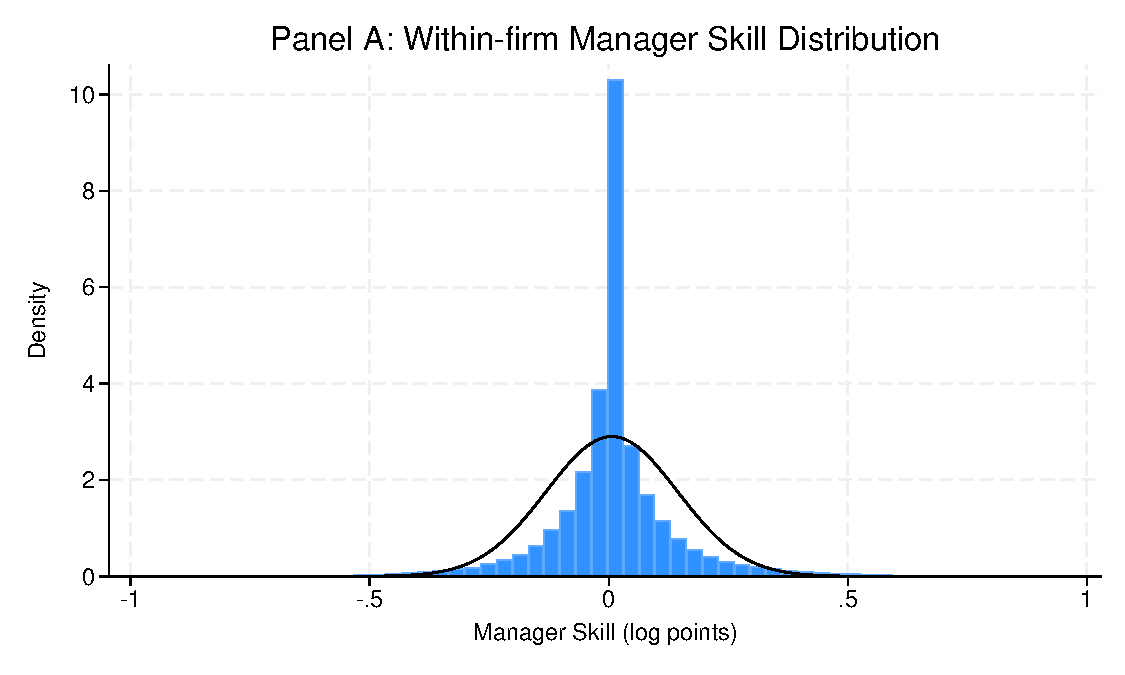
\includegraphics[width=\textwidth]{figure/manager_skill_within.pdf}
\end{minipage}
\hfill
\begin{minipage}{0.48\textwidth}
\centering
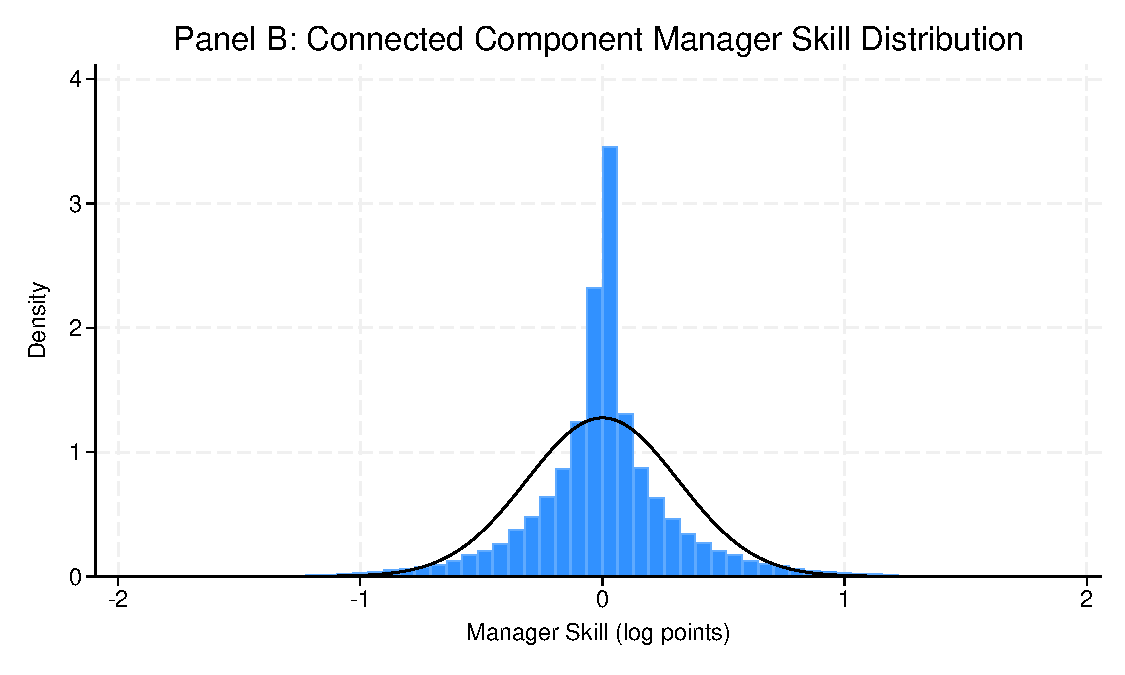
\includegraphics[width=\textwidth]{figure/manager_skill_connected.pdf}
\end{minipage}
\caption{Manager Skill Distributions}
\label{fig:manager_skills}
\footnotesize
Notes: Panel A shows the distribution of within-firm manager skill variation for firms with multiple CEOs. Panel B shows the distribution of manager skills in the largest connected component of managers. Both distributions show manager skills in log points after normalization and scaling.
\end{figure}

\begin{figure}[htbp]
\centering
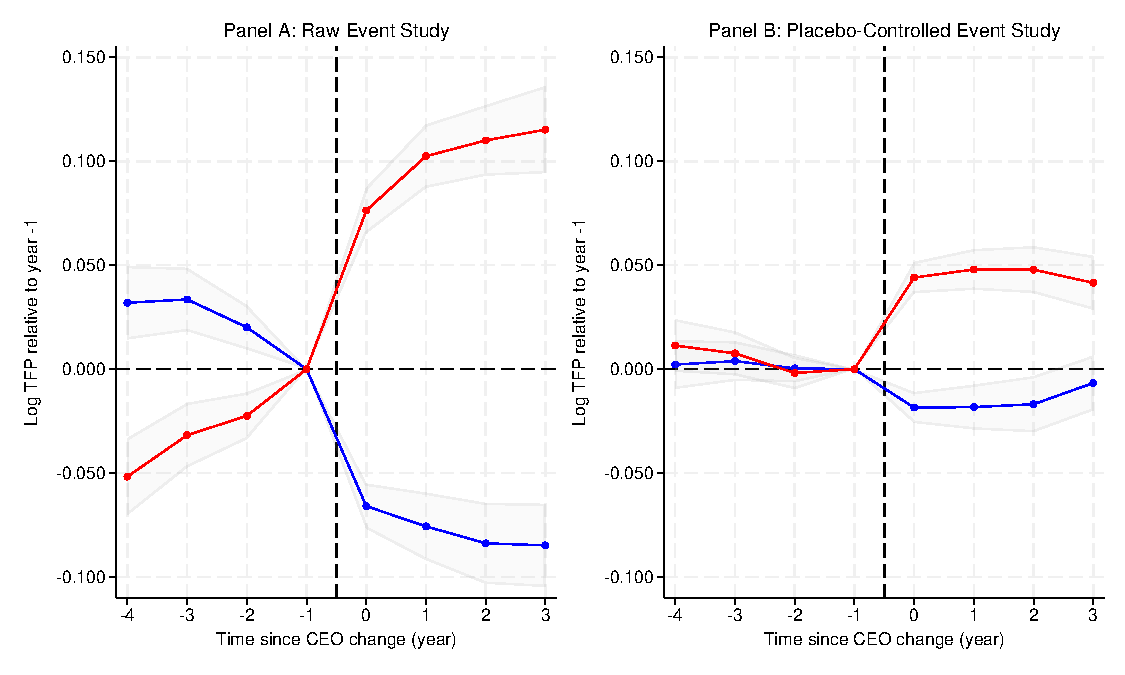
\includegraphics[width=0.8\textwidth]{figure/event_study.pdf}
\caption{Event Study: Impact of CEO Skill Changes on Firm Surplus}
\label{fig:event_study}
\footnotesize
Notes: Event study comparing firms that hire better managers (higher skill) versus worse managers (lower skill). The figure shows the difference in residual surplus between the two groups from 10 years before to 10 years after CEO transitions. Event time 0 represents the year of CEO change. Baseline period is 2 years before transition (event time -2). Gray shaded area represents 95\% confidence intervals. Sample includes 94,185 firms with exactly one CEO change during the observation period.
\end{figure}

\begin{table}[htbp]\centering
\def\sym#1{\ifmmode^{#1}\else\(^{#1}\)\fi}
\caption{Manager Skill Effects on Firm Outcomes}
\begin{tabular}{l*{3}{c}}
\toprule
                    &\multicolumn{1}{c}{(1)}&\multicolumn{1}{c}{(2)}&\multicolumn{1}{c}{(3)}\\
                    &\multicolumn{1}{c}{Revenue}&\multicolumn{1}{c}{EBITDA}&\multicolumn{1}{c}{Employment}\\
\midrule
Sales (log)         &       0.088\sym{***}&                     &                     \\
                    &     (0.005)         &                     &                     \\
\addlinespace
EBITDA (log)        &                     &       0.059\sym{***}&                     \\
                    &                     &     (0.005)         &                     \\
\addlinespace
Employment (log)    &                     &                     &       0.094\sym{***}\\
                    &                     &                     &     (0.009)         \\
\addlinespace
Constant            &      -0.882\sym{***}&      -0.463\sym{***}&      -0.090\sym{***}\\
                    &     (0.045)         &     (0.041)         &     (0.012)         \\
\midrule
Observations        &     1611007         &     1215276         &     1611007         \\
Adjusted R-squared  &       0.005         &       0.002         &       0.002         \\
\bottomrule
\multicolumn{4}{l}{\footnotesize Standard errors in parentheses}\\
\multicolumn{4}{l}{\footnotesize Standard errors clustered at firm level.}\\
\multicolumn{4}{l}{\footnotesize All regressions include industry-year fixed effects.}\\
\multicolumn{4}{l}{\footnotesize \sym{*} \(p<0.05\), \sym{**} \(p<0.01\), \sym{***} \(p<0.001\)}\\
\end{tabular}
\end{table}


\bibliographystyle{apacite}
\bibliography{references}

\appendix
\section{Robustness Checks}

\subsection{Placebo Event Study}

\begin{figure}[htbp]
\centering
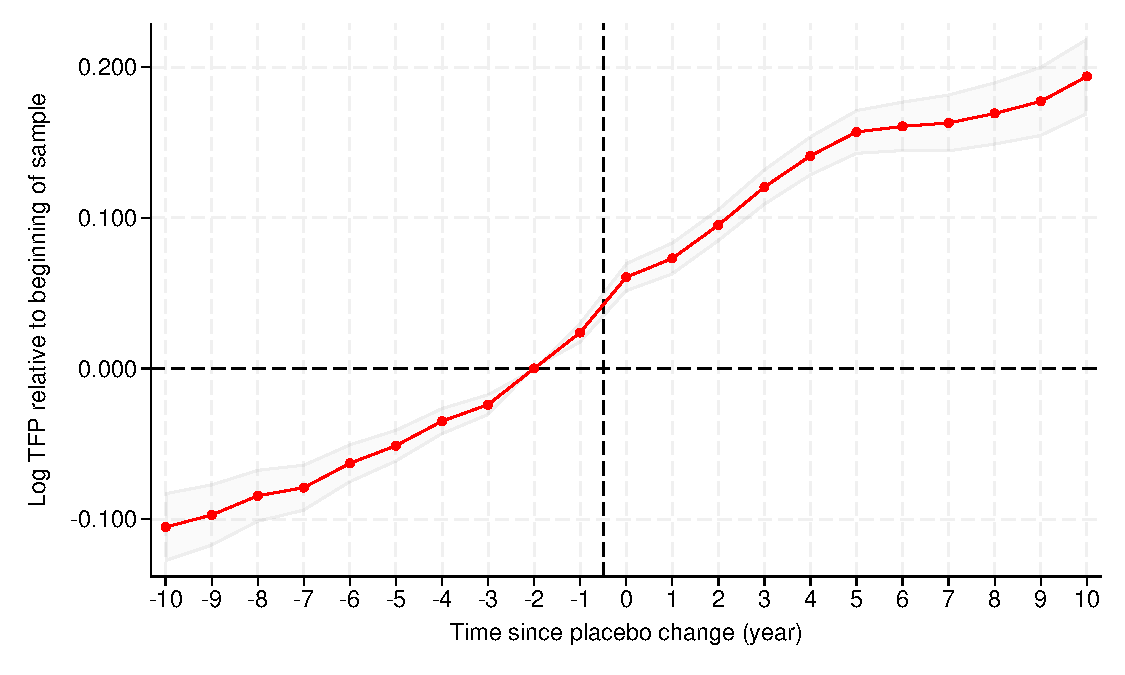
\includegraphics[width=0.8\textwidth]{figure/placebo.pdf}
\caption{Placebo Event Study: Random CEO Transition Timing}
\label{fig:placebo}
\footnotesize
Notes: Placebo event study with randomly assigned CEO transition times. For each firm experiencing an actual CEO change, we assign a placebo transition at a random year, excluding three years before and after the actual transition. The figure shows the difference in residual surplus between firms classified as hiring "better" versus "worse" managers based on skill changes at the placebo transition time. Event time 0 represents the placebo transition year. Baseline period is event time -2. Gray shaded area represents 95\% confidence intervals. The minimal differential effects validate that our main results capture the causal impact of actual CEO transitions rather than mechanical features of the methodology.
\end{figure}

Figure \ref{fig:placebo} presents the results of our placebo analysis. In stark contrast to the actual CEO transitions shown in Figure \ref{fig:event_study}, the placebo transitions exhibit virtually no differential performance effects. Firms randomly assigned to the "better" and "worse" manager categories show negligible differences in surplus throughout the event window, with point estimates close to zero and confidence intervals consistently overlapping. This null result for randomly timed transitions provides strong validation that the large effects in our main analysis reflect genuine CEO skill impacts rather than spurious correlations or methodological artifacts.

\begin{table}[htbp]\centering
\def\sym#1{\ifmmode^{#1}\else\(^{#1}\)\fi}
\caption{The revenue function in various samples}
\begin{tabular}{l*{5}{c}}
\hline\hline
                    &\multicolumn{1}{c}{(1)}&\multicolumn{1}{c}{(2)}&\multicolumn{1}{c}{(3)}&\multicolumn{1}{c}{(4)}&\multicolumn{1}{c}{(5)}\\
                    &\multicolumn{1}{c}{Full}&\multicolumn{1}{c}{sample}&\multicolumn{1}{c}{First CEO spell}&\multicolumn{1}{c}{Single CEO spell}&\multicolumn{1}{c}{Multiple CEO spells}\\
\hline
Tangible and intangible assets (log)&       0.254\sym{***}&       0.255\sym{***}&       0.256\sym{***}&       0.249\sym{***}&       0.275\sym{***}\\
                    &     (0.001)         &     (0.001)         &     (0.001)         &     (0.001)         &     (0.002)         \\
[1em]
Intangible assets share&      -0.028\sym{***}&      -0.027\sym{***}&      -0.038\sym{***}&      -0.016\sym{*}  &      -0.040\sym{***}\\
                    &     (0.007)         &     (0.009)         &     (0.011)         &     (0.010)         &     (0.014)         \\
[1em]
Foreign owned       &       0.012         &       0.012         &      -0.004         &       0.018\sym{*}  &       0.022         \\
                    &     (0.008)         &     (0.011)         &     (0.014)         &     (0.010)         &     (0.013)         \\
\hline
Observations        &     6634335         &     4404163         &     3073377         &     3560899         &     1797728         \\
\hline\hline
\multicolumn{6}{l}{\footnotesize Controls: firm-CEO-spell fixed effects; industry-year fixed effects.}\\
\end{tabular}
\end{table}


\begin{table}[htbp]\centering
\def\sym#1{\ifmmode^{#1}\else\(^{#1}\)\fi}
\caption{The revenue function by sector}
\begin{tabular}{l*{6}{c}}
\hline\hline
                    &\multicolumn{1}{c}{(1)}&\multicolumn{1}{c}{(2)}&\multicolumn{1}{c}{(3)}&\multicolumn{1}{c}{(4)}&\multicolumn{1}{c}{(5)}&\multicolumn{1}{c}{(6)}\\
                    &\multicolumn{1}{c}{Agriculture}&\multicolumn{1}{c}{Manufacturing}&\multicolumn{1}{c}{Wholesale, Retail, Transportation}&\multicolumn{1}{c}{Telecom and Business Services}&\multicolumn{1}{c}{Construction}&\multicolumn{1}{c}{Nontradable services}\\
\hline
Tangible and intangible assets (log)&       0.320\sym{***}&       0.296\sym{***}&       0.257\sym{***}&       0.237\sym{***}&       0.281\sym{***}&       0.207\sym{***}\\
                    &     (0.006)         &     (0.003)         &     (0.002)         &     (0.002)         &     (0.002)         &     (0.002)         \\
[1em]
Intangible assets share&       0.071         &       0.011         &      -0.006         &      -0.057\sym{***}&       0.029         &      -0.020         \\
                    &     (0.059)         &     (0.025)         &     (0.014)         &     (0.013)         &     (0.030)         &     (0.015)         \\
[1em]
Foreign owned       &      -0.070\sym{*}  &       0.046\sym{*}  &       0.008         &       0.082\sym{***}&      -0.055         &      -0.013         \\
                    &     (0.042)         &     (0.024)         &     (0.015)         &     (0.022)         &     (0.041)         &     (0.015)         \\
\hline
Observations        &      208269         &      748880         &     1893882         &     1224209         &      630073         &     1708957         \\
\hline\hline
\multicolumn{7}{l}{\footnotesize Controls: firm-CEO-spell fixed effects; industry-year fixed effects.}\\
\end{tabular}
\end{table}



\end{document}

% Available BibTeX keys from references.bib:
% McGrattan2012RED
% DeLoecker2011Econometrica
% AtkesonKehoe2005JPE
% Navaretti2010EFIGE
% Abowd1999Econometrica
% Card2018JoLE
% Bertrand2003-io
% Halpern2015-se
% Fisman2014-pw
% reghdfe
% greene
% cegtv
% frydman2010executive
% bandiera2020ceo
% Arnold2009-so
% bennedsen2020ceos
% Koren2017-rs
% Lucas1978-rp
% Syverson2011-ti
% cegjegyzek2024
% merleg2024
% McGrattanPrescott2008WP396
% Bloom2014-ux
% Callaway2021JoLE
% Koren2023expat
% Koren2024xt2treatments
